\thispagestyle{simple}
\chapter{Metodologia}\label{chap:metodologia}

Para alcançar os objetivos propostos neste trabalho, a metodologia de desenvolvimento foi baseada em 5 etapas, conforme ilustra a~\autoref{fig:fluxograma_metodologia}, a seguir:

\begin{figure}[!ht]
    \centering
    \caption{Fluxograma das etapas do trabalho.}\label{fig:fluxograma_metodologia}
    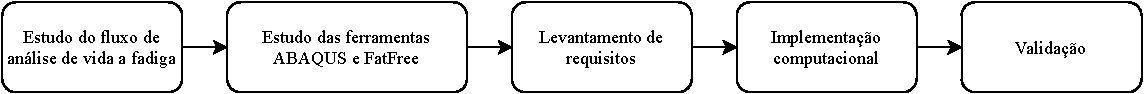
\includegraphics[width=\textwidth]{imagens/fluxograma_metodologia}
    \fonte{Autor (2021).}
\end{figure}

A primeira etapa consistiu em estudar o fluxo básico de trabalho de profissional, desde o acesso às informações até chegar nos resultados de fadiga. Essa etapa foi desenvolvida através de reuniões e oficinas ministrados por engenheiros da PETROBRAS que atuam na realização das análises de dutos em vão-livre (interessados diretos no desenvolvimento da ferramenta). Nessa etapa foram identificados as principais dificuldades do processo, destacando aqueles de maior potencial de automatização.

Em seguida, na segunda etapa, buscou-se conhecer os softwares que seriam integrados pela ferramenta: ABAQUS e FatFree. Com isso, pôde-se conhecer as oportunidades e limitações para integração de cada uma delas. %chktex 19

Na terceira etapa, fez-se a definição dos requisitos do sistema. Por exemplo: elaboração da especificação do fluxo dos dados na ferramenta, culminando na especificação de um arquivo de entrada para facilitar a estruturação dos dados para consumo pela aplicação. E assim chegou-se a um novo fluxo de trabalho que será apresentado mais adiante na~\autoref{sec:fluxo-com-ferramenta}.

Na quarta etapa, houve o desenvolvimento de uma série de \textit{scripts} em linguagem Python para automação de algumas tarefas.
Essa fase, de caráter exploratório, permitiu o desenvolvimento de pequenas ferramentas que podiam ter \textit{feedback} mais rápido, melhorando o entendimento dos requisitos e compressão da visão geral do fluxo de trabalho.
Com esse conjunto inicial de \textit{scripts}, fez-se então a modelagem dos módulos da aplicação com base nas diferentes funcionalidades previstas para a ferramenta.
Os códigos dos \textit{scripts} foram, então, reagrupados nesses módulos, que se comunicam por meio da utilização das diversas classes e respectivos métodos.

Finalmente, na quinta e última etapa, fez-se a validação da ferramenta usando dados de dutos reais da PETROBRAS\@.
No entanto, devido à confidencialidade destes dados, neste trabalho não serão apresentados os casos usados na validação, mas casos com dados fictícios para exemplificar as funcionalidades da ferramenta.